%% Copyright 2009 Ivan Griffin
%
% This State Transition Diagram (STD) contains the logic for
% the PC-brewing program. Every state contains a default set of
% actions, as listed in table 1. When a condition (green) is met, the
% transfer to another state is made. In that case, the resulting action (red)
% is performed.
%
% The structure for describing the STD is made in Latex / Tikz and is
% heavily based on the tcp_state_machine.tex document from Ivan Griffin,
% an example illustrating the TCP (RFC 793) state machine, 2009-11-20.
%-------------------------------------------------------------

%\documentclass{article}
\documentclass[border=5mm,tikz,preview,a3paper]{standalone}

\usepackage{tikz}
\usetikzlibrary{calc,backgrounds}
%\usepackage[active,tightpage]{preview}

\begin{document}
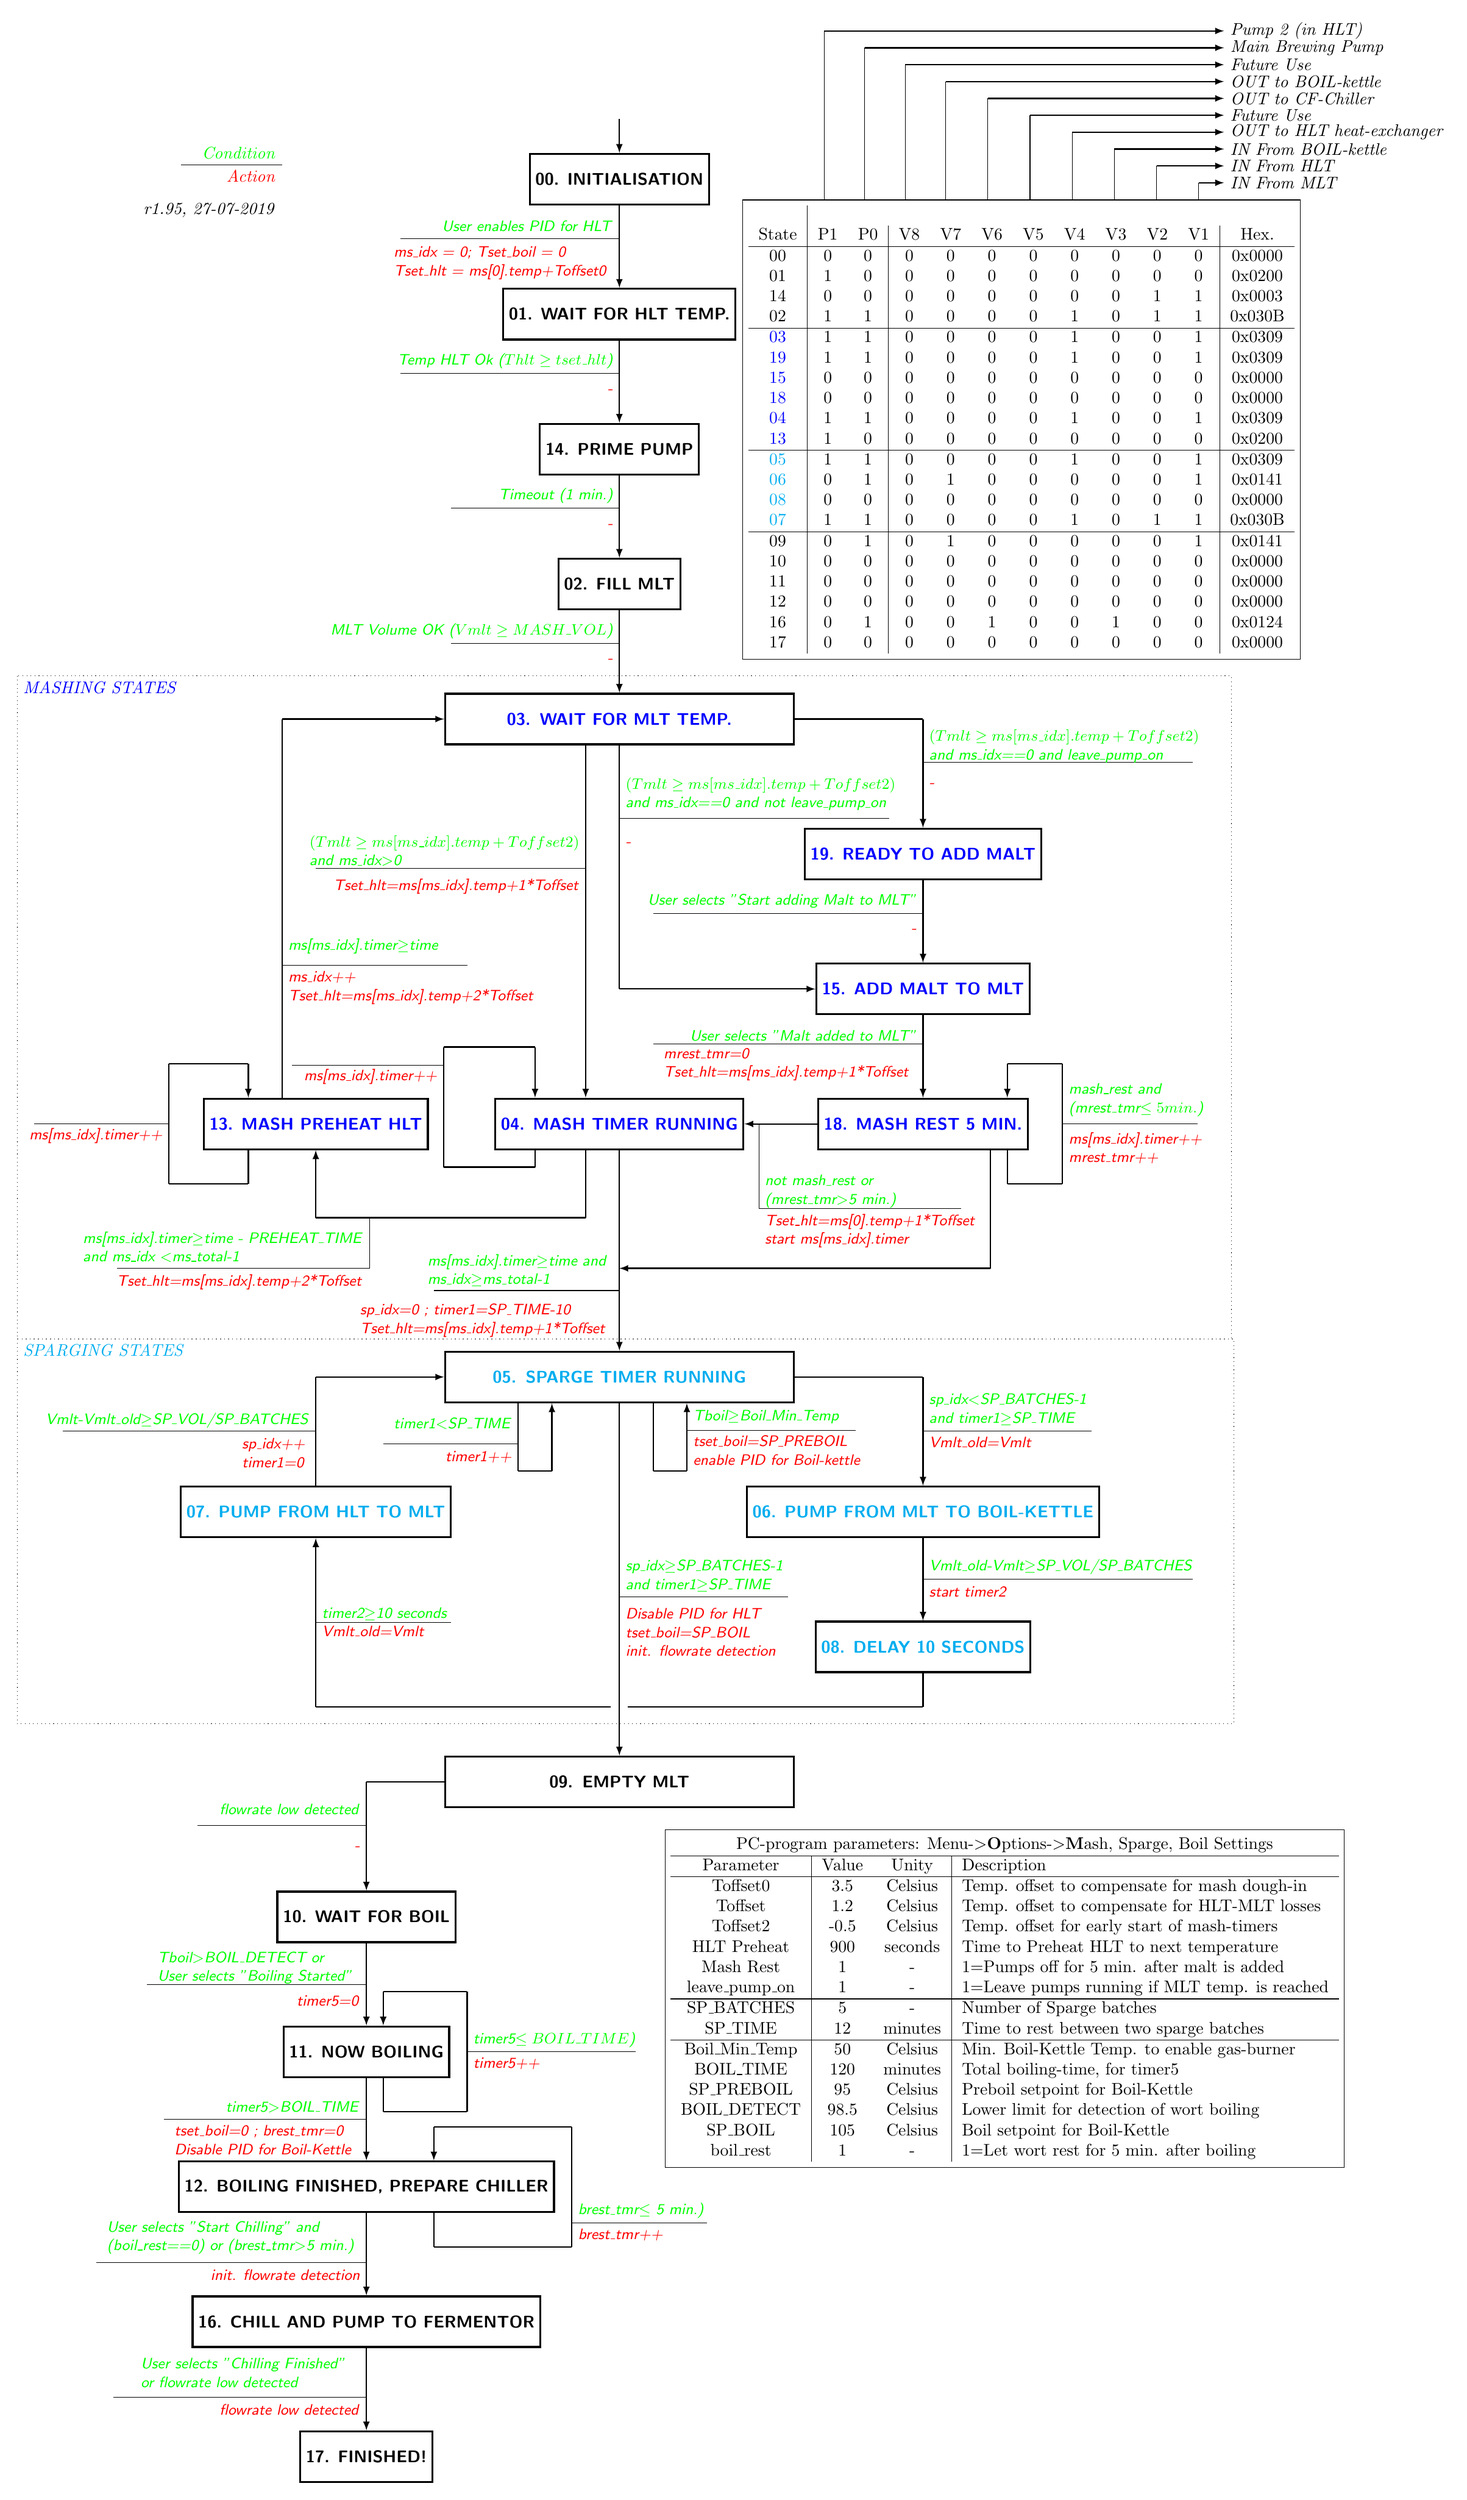
\begin{tikzpicture}[>=latex]
  % ----------------------------------
  % Styles for states, and state edges
  % ----------------------------------
  \tikzstyle{state} = [draw, very thick, fill=white, rectangle, minimum height=3em, minimum width=7em, node distance=8em, font={\sffamily\bfseries}]
  \tikzstyle{stateEdgePortion} = [black,thick];
  \tikzstyle{stateEdge} = [stateEdgePortion,->];
  \tikzstyle{edgeCondition} = [pos=0.4, left, green, font={\sffamily\small}];
  \tikzstyle{edgeAction} = [pos=0.6, left, red, font={\sffamily\small}];

  % ----------------
  % Position States
  % ----------------
  \node[state, name=std00]                                                                        {00. INITIALISATION};
  \node[state, name=std01,below of=std00]                                                         {01. WAIT FOR HLT TEMP.};
  \node[state, name=std14,below of=std01]                                                         {14. PRIME PUMP};
  \node[state, name=std02,below of=std14]                                                         {02. FILL MLT};
  \node[state, name=std03,below of=std02,text=blue,text width=20em,align=center]                  {03. WAIT FOR MLT TEMP.};
  \node[state, name=std19,below of=std03,right of=std03,xshift=10em,text=blue]                    {19. READY TO ADD MALT};
  \node[state, name=std15,below of=std19,text=blue]                                               {15. ADD MALT TO MLT};
  \node[state, name=std18,below of=std15,text=blue]                                               {18. MASH REST 5 MIN.};
  \node[state, name=std04,left  of=std18,xshift=-10em,text=blue]                                  {04. MASH TIMER RUNNING};
  \node[state, name=std13,left  of=std04,xshift=-10em,text=blue]                                  {13. MASH PREHEAT HLT};
  \node[state, name=std05,below of=std04,yshift=-7em,text=cyan,text width=20em,align=center]      {05. SPARGE TIMER RUNNING};
  \node[state, name=std06,below of=std05,right of=std05,xshift=10em,text=cyan]                    {06. PUMP FROM MLT TO BOIL-KETTLE};
  \node[state, name=std08,below of=std06,text=cyan]                                               {08. DELAY 10 SECONDS};
  \node[state, name=std07,left  of=std05,below of=std05,xshift=-10em,text=cyan]                   {07. PUMP FROM HLT TO MLT};
  \node[state, name=std09,below of=std05,left of=std08,xshift=-10em,text width=20em,align=center] {09. EMPTY MLT};
  \node[state, name=std10,below of=std09,left of=std09,xshift=-7em]                               {10. WAIT FOR BOIL};
  \node[state, name=std11,below of=std10]                                                         {11. NOW BOILING};
  \node[state, name=std12,below of=std11]                                                         {12. BOILING FINISHED, PREPARE CHILLER};
  \node[state, name=std16,below of=std12]                                                         {16. CHILL AND PUMP TO FERMENTOR};
  \node[state, name=std17,below of=std16]                                                         {17. FINISHED!};

  \node(std_bits)[shape=rectangle,draw,below of=std00,right of=std00,xshift=21em,yshift=-12em]
  {
  	\begin{tabular}{c|c c|c c c c c c c c|c} 
  	       \\ State & P1 & P0 & V8 & V7 & V6 & V5 & V4 & V3 & V2 & V1 & Hex.\\ \hline
	             00 & 0  & 0  & 0  & 0  & 0  & 0  & 0  & 0  & 0  & 0  & 0x0000\\
	             01 & 1  & 0  & 0  & 0  & 0  & 0  & 0  & 0  & 0  & 0  & 0x0200\\
	             14 & 0  & 0  & 0  & 0  & 0  & 0  & 0  & 0  & 1  & 1  & 0x0003\\
	             02 & 1  & 1  & 0  & 0  & 0  & 0  & 1  & 0  & 1  & 1  & 0x030B\\ \hline
	\color{blue} 03 & 1  & 1  & 0  & 0  & 0  & 0  & 1  & 0  & 0  & 1  & 0x0309\\
	\color{blue} 19 & 1  & 1  & 0  & 0  & 0  & 0  & 1  & 0  & 0  & 1  & 0x0309\\
	\color{blue} 15 & 0  & 0  & 0  & 0  & 0  & 0  & 0  & 0  & 0  & 0  & 0x0000\\
	\color{blue} 18 & 0  & 0  & 0  & 0  & 0  & 0  & 0  & 0  & 0  & 0  & 0x0000\\
	\color{blue} 04 & 1  & 1  & 0  & 0  & 0  & 0  & 1  & 0  & 0  & 1  & 0x0309\\
	\color{blue} 13 & 1  & 0  & 0  & 0  & 0  & 0  & 0  & 0  & 0  & 0  & 0x0200\\ \hline
	\color{cyan} 05 & 1  & 1  & 0  & 0  & 0  & 0  & 1  & 0  & 0  & 1  & 0x0309\\
	\color{cyan} 06 & 0  & 1  & 0  & 1  & 0  & 0  & 0  & 0  & 0  & 1  & 0x0141\\
	\color{cyan} 08 & 0  & 0  & 0  & 0  & 0  & 0  & 0  & 0  & 0  & 0  & 0x0000\\
	\color{cyan} 07 & 1  & 1  & 0  & 0  & 0  & 0  & 1  & 0  & 1  & 1  & 0x030B\\ \hline
	             09 & 0  & 1  & 0  & 1  & 0  & 0  & 0  & 0  & 0  & 1  & 0x0141\\
	             10 & 0  & 0  & 0  & 0  & 0  & 0  & 0  & 0  & 0  & 0  & 0x0000\\
	             11 & 0  & 0  & 0  & 0  & 0  & 0  & 0  & 0  & 0  & 0  & 0x0000\\
	             12 & 0  & 0  & 0  & 0  & 0  & 0  & 0  & 0  & 0  & 0  & 0x0000\\
	             16 & 0  & 1  & 0  & 0  & 1  & 0  & 0  & 1  & 0  & 0  & 0x0124\\
	             17 & 0  & 0  & 0  & 0  & 0  & 0  & 0  & 0  & 0  & 0  & 0x0000
	\end{tabular}
  };
  \draw ($(std_bits.north) + (-11.7em,0)$) -- ($(std_bits.north) + (-11.7em,10em)$)  %P1
	    edge[stateEdge] node[right,pos=1.0]{\emph{Pump 2 (in HLT)}} ($(std_bits.north) + (12em,10em)$) ;
  \draw ($(std_bits.north) + (-9.3em,0)$) -- ($(std_bits.north) + (-9.3em,9em)$)  %P0
	    edge[stateEdge] node[right,pos=1.0]{\emph{Main Brewing Pump}} ($(std_bits.north) + (12em,9em)$) ;
  \draw ($(std_bits.north) + (-6.9em,0)$)  -- ($(std_bits.north) + (-6.9em,8em)$)  %V8
		edge[stateEdge] node[right,pos=1.0]{\emph{Future Use}} ($(std_bits.north) + (12em,8em)$) ;
  \draw ($(std_bits.north) + (-4.5em,0)$)  -- ($(std_bits.north) + (-4.5em,7em)$)  %V7
		edge[stateEdge] node[right,pos=1.0]{\emph{OUT to BOIL-kettle}} ($(std_bits.north) + (12em,7em)$) ;
  \draw ($(std_bits.north) + (-2.0em,0)$)  -- ($(std_bits.north) + (-2.0em,6em)$)  %V6
		edge[stateEdge] node[right,pos=1.0]{\emph{OUT to CF-Chiller}} ($(std_bits.north) + (12em,6em)$) ;
  \draw ($(std_bits.north) + (0.5em,0)$)   -- ($(std_bits.north) + (0.5em,5em)$)   %V5
		edge[stateEdge] node[right,pos=1.0]{\emph{Future Use}} ($(std_bits.north) + (12em,5em)$) ;
  \draw ($(std_bits.north) + (3.0em,0)$)   -- ($(std_bits.north) + (3.0em,4em)$)   %V4
		edge[stateEdge] node[right,pos=1.0]{\emph{OUT to HLT heat-exchanger}} ($(std_bits.north) + (12em,4em)$) ;
  \draw ($(std_bits.north) + (5.5em,0)$)   -- ($(std_bits.north) + (5.5em,3em)$)   %V3
	    edge[stateEdge] node[right,pos=1.0]{\emph{IN From BOIL-kettle}} ($(std_bits.north) + (12em,3em)$) ;
  \draw ($(std_bits.north) + (8.0em,0)$)   -- ($(std_bits.north) + (8.0em,2em)$)   %V2
        edge[stateEdge] node[right,pos=1.0]{\emph{IN From HLT}} ($(std_bits.north) + (12em,2em)$) ;
  \draw ($(std_bits.north) + (10.5em,0)$)  -- ($(std_bits.north) + (10.5em,1em)$)  %V1
        edge[stateEdge] node[right,pos=1.0]{\emph{IN From MLT}}($(std_bits.north) + (12em,1em)$) ;
  
  \node(std_bits)[shape=rectangle,draw,below of=std09,right of=std09,xshift=20em,yshift=-10em]
  {
  	\begin{tabular}{c|c c|l}
  	     \multicolumn{4}{c}{PC-program parameters: Menu-\textgreater \textbf{O}ptions-\textgreater \textbf{M}ash, Sparge, Boil Settings}\\ \hline
  	     Parameter & Value & Unity & Description \\ \hline
  	     Toffset0  & 3.5   & Celsius & Temp. offset to compensate for mash dough-in   \\
  	     Toffset   & 1.2   & Celsius & Temp. offset to compensate for HLT-MLT losses  \\
  	     Toffset2  & -0.5  & Celsius & Temp. offset for early start of mash-timers    \\
  	   HLT Preheat & 900   & seconds & Time to Preheat HLT to next temperature        \\
  	     Mash Rest & 1     & -       & 1=Pumps off for 5 min. after malt is added     \\
   leave\_pump\_on & 1     & -       & 1=Leave pumps running if MLT temp. is reached  \\ \hline
	   SP\_BATCHES & 5     & -       & Number of Sparge batches                       \\
	   SP\_TIME    & 12    & minutes & Time to rest between two sparge batches        \\ \hline
   Boil\_Min\_Temp & 50    & Celsius & Min. Boil-Kettle Temp. to enable gas-burner    \\
	   BOIL\_TIME  & 120   & minutes & Total boiling-time, for timer5                 \\
	   SP\_PREBOIL & 95    & Celsius & Preboil setpoint for Boil-Kettle               \\
     BOIL\_DETECT  & 98.5  & Celsius & Lower limit for detection of wort boiling      \\
	      SP\_BOIL & 105   & Celsius & Boil setpoint for Boil-Kettle                  \\
	   boil\_rest  & 1     & -       & 1=Let wort rest for 5 min. after boiling       
  	\end{tabular} 
  };

  % ------------------------
  % Connect States via edges
  % ------------------------
  % General stuff
  \draw ($(std00.north) + (-20em,0)$)      node[left,green]{\emph{Condition}}
        ($(std00.north) + (-20em,-1.4em)$) node[left,red]{\emph{Action}}
        ($(std00.north) + (-20em,-3.4em)$) node[left]{\emph{r1.95, 27-07-2019}}
        ($(std00.north) + (-26em,-0.7em)$) -- ($(std00.north) + (-20em,-0.7em)$)
        ($(std00.north) + (0,2em)$)        edge[stateEdge] (std00.north) ; % to 00 (power-up)

  % From 00. Initialisation
  \draw % To 01. Wait for HLT Temp.
        (std00.south)        edge[stateEdge] 
                             node[edgeCondition, pos=0.25]{\emph{User enables PID for HLT}} 
                             node[edgeAction, text width=13em, pos=0.7]{\emph{ms\_idx = 0; Tset\_boil = 0\\Tset\_hlt = ms[0].temp+Toffset0}}
                             coordinate[pos=0.40] (A1) (std01.north) 
        ($(A1) + (-13em,0)$) -- (A1) 
        ;

  % From 01. Wait for HLT Temp.
  \draw % To 02. Prime Pump
        (std01.south)        edge[stateEdge] 
                             node[edgeCondition, pos=0.25]{\emph{Temp HLT Ok  ($Thlt\ge tset\_hlt$)}}
                             node[edgeAction]{\emph{-}}
                             coordinate[pos=0.40] (A2) (std14.north) 
	    ($(A2) + (-13em,0)$) -- (A2) 
	    ;

  % From 14. Prime Pump
   \draw % To 02. Fill MLT
         (std14.south)        edge[stateEdge] 
                              node[edgeCondition, pos=0.25]{\emph{Timeout (1 min.)}} 
                              node[edgeAction]{\emph{-}}
                              coordinate[pos=0.40] (A3) (std02.north) 
         ($(A3) + (-10em,0)$) -- (A3) 
         ;

  % From 02. Fill MLT
  \draw % To 03. Wait for MLT Temp.
        (std02.south)        edge[stateEdge] 
                             node[edgeCondition, pos=0.25]{\emph{MLT Volume OK ($Vmlt\ge MASH\_VOL$)}} 
                             node[edgeAction]{\emph{-}}
                             coordinate[pos=0.40] (A4) (std03.north) 
        ($(A4) + (-10em,0)$) -- (A4) 
        ;

  % From 03. Wait for MLT Temp.
  \coordinate (A031) at (std03.east -| std19.north) ;
  \coordinate (A032) at (std03.south |- std15.east) ;
  \draw % To state 19. Ready to add Malt
        (std03.east)         edge[stateEdgePortion] (A031)
        (A031)               edge[stateEdge] 
                             node[edgeCondition,right,text width=16em,pos=0.25]{\emph{$(Tmlt\ge ms[ms\_idx].temp+Toffset2)$ \\and ms\_idx==0 and leave\_pump\_on}} 
                             node[edgeAction,right]{\emph{-}} coordinate[pos=0.40] (A6) (std19.north) 
        ($(A6) + (+16em,0)$) -- (A6) 

        % To state 15. Add Malt to MLT
        (std03.south)        edge[stateEdgePortion]
                             node[edgeCondition,right,text width=16em,pos=0.2]{\emph{$(Tmlt\ge ms[ms\_idx].temp+Toffset2)$ \\and ms\_idx==0 and not leave\_pump\_on}} 
                             node[edgeAction,right,pos=0.4]{\emph{-}} coordinate[pos=0.30] (A6) (A032)       
        (A032)               edge[stateEdge] (std15.west) 
        ($(A6) + (+16em,0)$) -- (A6)        
         
        % To state 04. Mash Timer Running
		($(std03.south) + (-2em,0)$) edge[stateEdge] 
		                             node[edgeCondition,left,text width=16em,pos=0.3]{\emph{$(Tmlt\ge ms[ms\_idx].temp+Toffset2)$ \\and ms\_idx\textgreater0}} 
		                             node[edgeAction,left,pos=0.4]{\emph{Tset\_hlt=ms[ms\_idx].temp+1*Toffset}} coordinate[pos=0.35] (A61) ($(std04.north) + (-2em,0)$)
		($(A61) + (-16em,0)$)        -- (A61) 
		;        
		                             
   % From 19. Ready to Add Malt 
   \draw (std19.south)        edge[stateEdge] 
 					          node[edgeCondition, pos=0.25]{\emph{User selects "Start adding Malt to MLT"}} 
 					          node[edgeAction]{\emph{-}}
 					          coordinate[pos=0.40] (A7) (std15.north) 
         ($(A7) + (-16em,0)$) -- (A7) 
         ;

   % From 15. Add Malt to MLT
   \draw % To state 18. Mash rest 5 min.
         (std15.south)        edge[stateEdge] 
					          node[edgeCondition, pos=0.25]{\emph{User selects "Malt added to MLT"}} 
					          node[edgeAction,text width=15em]{\emph{mrest\_tmr=0\\Tset\_hlt=ms[ms\_idx].temp+1*Toffset}} coordinate[pos=0.35] (A8) (std18.north) 
	     ($(A8) + (-16em,0)$) -- (A8) 
	     ;

   % From 18. Mash rest 5 Min.
   \coordinate (A18NE) at ($(std18.north -| std18.east) + (2em,2em)$) ;
   \coordinate (A18SE) at ($(std18.south -| std18.east) + (2em,-2em)$) ;
   \coordinate (S1805) at ($(std18.south) + (4em,-7em)$) ;
   \coordinate (S1806) at ($(std05.north) + (0,2em)$) ;
   \draw % To itself (right)
         ($(std18.south) + (5em,0)$)        edge[stateEdgePortion]       ($(std18.south) + (5em,-2em)$) 
         ($(std18.south) + (5em,-2em)$)     edge[stateEdgePortion]       (A18SE) 
         (A18SE)                            edge[stateEdgePortion] 
                                            node[edgeCondition,pos=0.7,right,text width=8em]{\emph{mash\_rest and\\(mrest\_tmr$\le 5 min.$)}} 
                                            node[edgeAction,pos=0.3,right,text width=10em]{\emph{ms[ms\_idx].timer++\\mrest\_tmr++}} 
                                            coordinate[pos=0.50] (A182)  (A18NE)
         (A18NE)                            edge[stateEdgePortion]       ($(std18.north) + (5em,2em)$) 
         ($(std18.north) + (5em,2em)$)      edge[stateEdge]              ($(std18.north) + (5em,0)$) 
         ($(A182) + (8em,0)$)               --                           (A182) 

         % To state 04. Mash Timer Running
         (std18.west)                       edge[stateEdge] coordinate[pos=0.80] (A18W) (std04.east) 
         ($(A18W) + (0,-5em)$)              -- 
                                            node[edgeCondition, right,pos=0.2,text width=10em]{\emph{not mash\_rest or\\(mrest\_tmr\textgreater 5 min.)}}                      (A18W) 
         ($(A18W) + (0,-5em)$)              -- 
                                            node[edgeAction,pos=0.0,below right,text width=13em]{\emph{Tset\_hlt=ms[0].temp+1*Toffset\\start ms[ms\_idx].timer}}          ($(A18W) + (+12em,-5em)$)

         % To state 05. Sparge Timer Running
         ($(std18.south) + (4em,0)$)        edge[stateEdgePortion]       (S1805)
         (S1805)                            edge[stateEdge]              (S1805 -| S1806)
         ;

   % From 04. Mash Timer running
   \coordinate (A4SW) at ($(std04.south -| std04.west) + (-3em,-1em)$) ;
   \coordinate (A4NW) at ($(std04.north -| std04.west) + (-3em,+3em)$) ;
   \coordinate (A413) at ($(std04.south -| std13.south) + (0,-4em)$) ;
   \draw % To itself (left)
         ($(std04.south) + (-5em,0)$)    edge[stateEdgePortion] ($(std04.south) + (-5em,-1em)$)
         ($(std04.south) + (-5em,-1em)$) edge[stateEdgePortion] (A4SW)
         (A4SW)                          edge[stateEdgePortion] 
                                         node[edgeAction,pos=0.75,left]{\emph{ms[ms\_idx].timer++}}
                                         coordinate[pos=0.85] (A44) (A4NW)
         (A4NW)                          edge[stateEdgePortion] ($(std04.north) + (-5em,+3em)$)
         ($(std04.north) + (-5em,+3em)$) edge[stateEdge]        ($(std04.north) + (-5em,0)$) 
         ($(A44) + (-9em,0)$)            -- (A44)
                                          

         % To state 5. Sparge Timer Running
         (std04.south)                   edge[stateEdge] 
		 			                     node[edgeCondition, pos=0.6,text width=11em]{\emph{ms[ms\_idx].timer$\ge$time and\\ms\_idx$\ge$ms\_total-1}} 
		 			                     node[edgeAction, text width=15em, pos=0.85]{\emph{sp\_idx=0 ; timer1=SP\_TIME-10\\Tset\_hlt=ms[ms\_idx].temp+1*Toffset}} coordinate[pos=0.70] (A041)  (std05.north) 
		 ($(A041) + (-11em,0)$)          --                          (A041)

		 % To state 13. Mash Preheat HLT
		 ($(std04.south) + (-2em,0)$)    edge[stateEdgePortion]      ($(std04.south) + (-2em,-4em)$)
		 ($(std04.south) + (-2em,-4em)$) edge[stateEdgePortion] coordinate[pos=0.80] (A4213) (A413)
		 (A413)                          edge[stateEdge]             (std13.south)
         (A4213)                         -- ($(A4213) + (0,-3em)$) -- 
                                         node[edgeCondition, pos=0.4,above,text width=22em]{\emph{ms[ms\_idx].timer$\ge$time - PREHEAT\_TIME\\ and ms\_idx \textless ms\_total-1}} 
                                         node[edgeAction, text width=9em, below,pos=0.7]{\emph{Tset\_hlt=ms[ms\_idx].temp+2*Toffset}} ($(A4213) + (-15em,-3em)$) 
         ;
         
   % From 13. Mash Preheat HLT
   \coordinate (A13SW) at ($(std13.south -| std13.west) + (-2em,-2em)$) ;
   \coordinate (A13NW) at ($(std13.north -| std13.west) + (-2em,+2em)$) ;
   \coordinate (S1303) at ($(std13.north |- std03.west) + (-2em,0)$) ;
   \draw % to itself (left)
         ($(std13.south) + (-4em,0)$)    edge[stateEdgePortion] ($(std13.south) + (-4em,-2em)$)
         ($(std13.south) + (-4em,-2em)$) edge[stateEdgePortion] (A13SW)
         (A13SW)                         edge[stateEdgePortion] 
                                         node[edgeAction,left,pos=0.4]{\emph{ms[ms\_idx].timer++}}
                                         coordinate[pos=0.50] (A131) (A13NW)
         (A13NW)                         edge[stateEdgePortion] ($(std13.north) + (-4em,+2em)$)
         ($(std13.north) + (-4em,+2em)$) edge[stateEdge]        ($(std13.north) + (-4em,0)$)                            
         ($(A131) + (-8em,0)$) --        (A131)

         % To state 03. Wait for MLT Temp.
         ($(std13.north) + (-2em,0)$)    edge[stateEdgePortion] 
                                         node[edgeCondition,right,text width=16em]{\emph{ms[ms\_idx].timer$\ge$time}} 
   									     node[edgeAction,right,pos=0.29,text width=11em]{\emph{ms\_idx++\\Tset\_hlt=ms[ms\_idx].temp+2*Toffset}}
                                         coordinate[pos=0.35] (A13) (S1303)
         (S1303)                         edge[stateEdge]            (std03.west)
         ($(A13) + (11em,0)$)           -- (A13) 
         ;
  
  % From 05. Sparge Timer Running
  \draw % To itself 1
        ($(std05.south) + (2em,0)$)      edge[stateEdgePortion] ($(std05.south) + (2em,-4em)$)
        ($(std05.south) + (2em,-4em)$)   edge[stateEdgePortion] ($(std05.south) + (4em,-4em)$)
        ($(std05.south) + (4em,-4em)$)   edge[stateEdge]  
                                         node[edgeCondition,right,pos=0.8]{\emph{Tboil$\ge$Boil\_Min\_Temp}}       
                                         node[edgeAction,right,text width=15em,pos=0.3]{\emph{tset\_boil=SP\_PREBOIL\\enable PID for Boil-kettle}}
                                         coordinate[pos=0.6] (A05L) ($(std05.south) + (4em,0)$)
        ($(A05L) + (10em,0)$)           -- (A05L)                                

        % To itself 2
        ($(std05.south) + (-6em,0)$)     edge[stateEdgePortion] 
                                         node[edgeCondition,left,pos=0.3]{\emph{timer1\textless SP\_TIME}}       
        								 node[edgeAction,left,pos=0.8]{\emph{timer1++}}
        								 coordinate[pos=0.6] (A05M) ($(std05.south) + (-6em,-4em)$)
        ($(std05.south) + (-6em,-4em)$)  edge[stateEdgePortion]     ($(std05.south) + (-4em,-4em)$)
        ($(std05.south) + (-4em,-4em)$)  edge[stateEdge]            ($(std05.south) + (-4em,0)$) 
        ($(A05M) + (-8em,0)$)            -- (A05M)
          
        % To state 06. Pump from MLT to Boil-Kettle
		(std05.east)                     edge[stateEdgePortion]     (std05.east -| std06.north)  
		(std05.east -| std06.north)      edge[stateEdge]            
		                                 node[edgeCondition,right,pos=0.3,text width=15em]{\emph{sp\_idx\textless SP\_BATCHES-1\\and timer1$\ge$SP\_TIME}}       
		                                 node[edgeAction,right,pos=0.6]{\emph{Vmlt\_old=Vmlt}}
		                                 coordinate[pos=0.5] (A05N)   (std06.north)  
        ($(A05N) + (10em,0)$)            -- (A05N)
        
        % To state 09. Empty MLT
		(std05.south)                    edge[stateEdge]     
										 node[edgeCondition,right,pos=0.49,text width=15em]{\emph{sp\_idx$\ge$SP\_BATCHES-1\\and timer1$\ge$SP\_TIME}}
										 node[edgeAction,right,pos=0.65,text width=15em]{\emph{Disable PID for HLT\\tset\_boil=SP\_BOIL\\init. flowrate detection}}
										 coordinate[pos=0.55] (A05P)   (std09.north)  
		($(A05P) + (10em,0)$)            -- (A05P)
        ;

  % From 06. Pump from MLT to Boil-Kettle
  \draw % To state 08. Delay 10 seconds
        (std06.south)         edge[stateEdge]            
                              node[edgeCondition,right,pos=0.35]{\emph{Vmlt\_old-Vmlt$\ge$SP\_VOL/SP\_BATCHES}}       
                              node[edgeAction,right,pos=0.65]{\emph{start timer2}}
                              coordinate[pos=0.5] (A06L)   (std08.north)  
        ($(A06L) + (16em,0)$) -- (A06L)
        ;

  % From 08. Delay 10 seconds
  %\coordinate (A4SW) at ($(std04.south -| std04.west) + (-3em,-2em)$) ;
  \coordinate (A8X) at ($(std08.south -| std05.south) + (0,-2em)$) ;
  \draw % To state 07. Pump from HLT to MLT
        (std08.south)                edge[stateEdgePortion] ($(std08.south) + (0,-2em)$)
        ($(std08.south) + (0,-2em)$) edge[stateEdgePortion] ($(A8X) + (0.5em,0)$)            
        ($(A8X) + (-0.5em,0)$)       edge[stateEdgePortion] (A8X -| std07.south)
        (A8X -| std07.south)         edge[stateEdge]
                                     node[edgeCondition,right,pos=0.55]{\emph{timer2$\ge$10 seconds}}       
                                     node[edgeAction,right,pos=0.45]{\emph{Vmlt\_old=Vmlt}}
                                     coordinate[pos=0.5] (A08L)   (std07.south)  
        ($(A08L) + (8em,0)$)         -- (A08L)
        ;
  
  % From state 07. Pump from HLT to MLT
  \draw % To state 05. Sparge Timer Running
        (std07.north)               edge[stateEdgePortion] 
                                    node[edgeCondition,left,pos=0.6]{\emph{Vmlt-Vmlt\_old$\ge$SP\_VOL/SP\_BATCHES}}       
                                    node[edgeAction,left,pos=0.3,text width=4em]{\emph{sp\_idx++\\timer1=0}}
                                    coordinate[pos=0.5] (A07L) (std07.north |- std05.west)            
        (std07.north |- std05.west) edge[stateEdge]            (std05.west)
        ($(A07L) + (-15em,0)$) -- (A07L)
        ;

  % From 09. Empty MLT
  \draw % To state 10. Wait for Boil
        (std09.west)                edge[stateEdgePortion] (std09.west -| std10.north) 
        (std09.west -| std10.north) edge[stateEdge]
                                    node[edgeCondition, pos=0.25]{\emph{flowrate low detected}} 
                                    node[edgeAction]{\emph{-}}
					  		        coordinate[pos=0.40] (A09L) (std10.north) 
		($(A09L) + (-10em,0)$)      -- (A09L) 
		;

  % From 10. Wait for Boil
  \draw (std10.south)          edge[stateEdge] 
							   node[edgeCondition,pos=0.3,text width=12em]{\emph{Tboil\textgreater BOIL\_DETECT or\\User selects "Boiling Started"}} 
							   node[edgeAction,pos=0.7]{\emph{timer5=0}}
							   coordinate[pos=0.5] (A10L) (std11.north) 
		($(A10L) + (-13em,0)$) -- (A10L) 
		;

  % From 11. Now Boiling
  \coordinate (A11NE) at ($(std11.north -| std11.east) + (1em,2em)$) ;
  \coordinate (A11SE) at ($(std11.south -| std11.east) + (1em,-2em)$) ;
  \draw % To itself (right)
          ($(std11.south) + (1em,0)$)        edge[stateEdgePortion]       ($(std11.south) + (1em,-2em)$) 
		  ($(std11.south) + (1em,-2em)$)     edge[stateEdgePortion]       (A11SE) 
		  (A11SE)                            edge[stateEdgePortion] 
											 node[edgeCondition,pos=0.6,right]{\emph{timer5$\le BOIL\_TIME$)}} 
											 node[edgeAction,pos=0.4,right,text width=10em]{\emph{timer5++}} 
											 coordinate[pos=0.50] (A112)  (A11NE)
		  (A11NE)                            edge[stateEdgePortion]       ($(std11.north) + (1em,2em)$) 
		  ($(std11.north) + (1em,2em)$)      edge[stateEdge]              ($(std11.north) + (1em,0)$) 
		  ($(A112) + (10em,0)$)              --                           (A112) 

        % To state 12. Boiling Finished, prepare Chiller
        (std11.south)          edge[stateEdge] 
							   node[edgeCondition,pos=0.35]{\emph{timer5\textgreater BOIL\_TIME}} 
							   node[edgeAction,pos=0.75,text width=11em]{\emph{tset\_boil=0 ; brest\_tmr=0\\Disable PID for Boil-Kettle}}
							   coordinate[pos=0.5] (A11L) (std12.north) 
		($(A11L) + (-12em,0)$) -- (A11L) 
		;

  % From 12. Boiling Finished, prepare Chiller
  \coordinate (A12NE) at ($(std12.north -| std12.east) + (1em,2em)$) ;
  \coordinate (A12SE) at ($(std12.south -| std12.east) + (1em,-2em)$) ;
  \draw % To itself (right)
          ($(std12.south) + (4em,0)$)        edge[stateEdgePortion]       ($(std12.south) + (4em,-2em)$) 
		  ($(std12.south) + (4em,-2em)$)     edge[stateEdgePortion]       (A12SE) 
		  (A12SE)                            edge[stateEdgePortion] 
										 	 node[edgeCondition,pos=0.3,right]{\emph{brest\_tmr$\le$ 5 min.)}} 
											 node[edgeAction,pos=0.1,right,text width=10em]{\emph{brest\_tmr++}} 
											 coordinate[pos=0.2] (A122)   (A12NE)
		  (A12NE)                            edge[stateEdgePortion]       ($(std12.north) + (4em,2em)$) 
		  ($(std12.north) + (4em,2em)$)      edge[stateEdge]              ($(std12.north) + (4em,0)$) 
		  ($(A122) + (8em,0)$)               --                           (A122) 
  
        % To state 16. Chill and Pump to Fermentor
        (std12.south)          edge[stateEdge] 
							   node[edgeCondition,pos=0.3,text width=15em]{\emph{User selects "Start Chilling" and\\(boil\_rest==0) or (brest\_tmr\textgreater 5 min.)}} 
							   node[edgeAction,pos=0.75]{\emph{init. flowrate detection}}
							   coordinate[pos=0.6] (A12L) (std16.north) 
        ($(A12L) + (-16em,0)$) -- (A12L) 
        ;

  % From 16. Chill and Pump to Fermentor
  \draw (std16.south)          edge[stateEdge] 
							   node[edgeCondition,pos=0.3,text width=13em]{\emph{User selects "Chilling Finished"\\or flowrate low detected}} 
							   node[edgeAction,pos=0.75]{\emph{flowrate low detected}}
							   coordinate[pos=0.6] (A17L) (std17.north) 
      ($(A17L) + (-15em,0)$) -- (A17L) 
      ;

  % draw dotted lines around passive and active closes
  \begin{pgfonlayer}{background}
  \draw [join=round,black,dotted] ($(std13.west |- std03.north) + (-11em,+1em)$) 
                                  node[below right,blue]{\emph{MASHING STATES}}
                                  rectangle ($(std18.south east) + (12em,-11.2em)$) ;
  \draw [join=round,black,dotted] ($(std13.west |- std05.north) + (-11em,+0.7em)$) 
								  node[below right,cyan]{\emph{SPARGING STATES}}
								  rectangle ($(std08.south east) + (12em,-3em)$) ;
  \end{pgfonlayer}

\end{tikzpicture}
\end{document}